% Numbered citation style: all seven Neurocomputing samples
% inspected use [n], none use author-year.
\documentclass[preprint,11pt]{elsarticle}

\usepackage{amsmath,amssymb}
\usepackage{graphicx}
\usepackage{booktabs}
\usepackage{multirow}
\usepackage{xcolor}
\usepackage[hidelinks,hypertexnames=false]{hyperref}
\usepackage{subcaption}
\usepackage{placeins}
\usepackage{tikz}
\usetikzlibrary{arrows.meta,positioning}

% --- Stable terminology. Use these everywhere; do not inline synonyms. ---
\newcommand{\tokenlevel}{token-level}
\newcommand{\modlevel}{modality-level}
\newcommand{\IMM}{\textsc{tok}}          % intra-modal (token) erasure
\newcommand{\FMM}{\textsc{mod}}          % whole-modality absence
\newcommand{\cleanacc}{clean-input accuracy}
\newcommand{\degr}{\ensuremath{\Delta_{\mathrm{clean}}}}  % clean-input change
\newcommand{\shiftgap}{\ensuremath{\Delta_{\mathrm{shift}}}}
% indexed form; never write \shiftgap_j -- that nests subscripts
\newcommand{\shiftgapj}[1]{\ensuremath{\Delta_{\mathrm{shift},#1}}}

\journal{Neurocomputing}

% Preserve the journal footer without the class's trailing interword glue.
\makeatletter
\def\ps@pprintTitle{%
  \let\@oddhead\@empty\let\@evenhead\@empty
  \def\@oddfoot{\hbox to \textwidth{\footnotesize\itshape
    Preprint submitted to \@journal\hfill\@date}}%
  \let\@evenfoot\@oddfoot}
\makeatother

\begin{document}

\begin{frontmatter}

\title{Token-Level Missingness Training Can Erode\\
       Clean-Input Performance in Multimodal Learning}

% Author block.
% Campus confirmed Boston by the author (2026-09-16).
% ORCID: omitted per author instruction.
\author[a]{Zehao Li}
\ead{li.zehao5@northeastern.edu}
\affiliation[a]{organization={Northeastern University},
                city={Boston}, state={MA}, country={USA}}

\begin{abstract}
Training for missing modalities can change a multimodal system's performance
even when every input is available. Temporal erasure and whole-modality
dropout expose the model to different observations and reconstruction signals,
although both are specified by a missing rate. We compare these training
protocols through their clean-input accuracy under benign and text-scarce
training regimes, using matched nominal rate schedules and a shared fusion
architecture with availability-gated reconstruction. Across CMU-MOSI,
CMU-MOSEI and CH-SIMS, text-scarce token-level
training reduces accuracy by up to $27.7$ percentage points relative to benign
training; the largest corresponding decrease under modality-level training is
$2.2$ points. In a rate sweep, the token-level decline is first more than two
percentage points at $50$--$60\%$ text erasure,
and subsampling CMU-MOSEI produces larger changes at smaller sample sizes.
The result replicates with BERT and RoBERTa; an \texttt{[UNK]}-substitution
control produces a $29.6$-point decrease. In intervention experiments,
modality-level training keeps clean-input accuracy close to the benign-regime
reference, while freezing lower layers or reducing the text-encoder learning
rate does not recover the token-level result. A separate 40-run control finds
a $23.0$-point token-level decrease even with auxiliary reconstruction loss
removed, compared with $1.1$ points under modality-level training.
These findings show that matched
nominal missing rates can produce different clean-input outcomes within a
shared architecture, motivating explicit evaluation of complete inputs
alongside missing-input robustness.
\end{abstract}

\begin{keyword}
incomplete multimodal learning \sep missing modalities \sep
multimodal sentiment analysis \sep fine-tuning dynamics \sep
clean-input performance
\end{keyword}

\end{frontmatter}

%======================================================================
\section{Introduction}
%======================================================================

Multimodal sentiment systems must remain useful when text, audio or video is
unavailable. For example, a transcription service can fail during an otherwise
intact audiovisual interaction and later resume. The system must handle both
the interruption and the return of complete inputs. Training pipelines prepare
for this condition by simulating
missingness. One common protocol erases temporal positions within a modality,
leaving a partially observed stream; we call it \tokenlevel{} missingness
(\IMM{}). Another removes a complete stream; we call it \modlevel{}
missingness (\FMM{}). Both are parameterised by a missing rate and are often
reported as alternative implementations of the same experimental condition.

Complete-input performance is already a concern in robust multimodal
learning~\cite{hazarika2022,missmodal}. The question here is how it changes
across training protocols as simulated missingness increases. A
complete-input score from a separately trained model, as in the complete and
incomplete settings of EMT-DLFR~\cite{emtdlfr}, does not answer that question.
We therefore compare models trained under benign and text-scarce missingness
on the same unmasked test inputs.

Our central measurement is the \emph{clean-input change}: the difference in
complete-input accuracy between text-scarce and benign missingness training.
At matched nominal rate schedules,
the two protocols separate sharply. \tokenlevel{} training changes clean-input
binary accuracy by as much as $-27.7$ points on CMU-MOSI, while \modlevel{}
training decreases it by no more than $2.2$ points in the corresponding comparisons.
The rate sweep identifies the first token-level declines of more than two
percentage points at text-erasure rates of $50$--$60\%$,
placing the effect inside the range used by published missing-modality
studies~\cite{emtdlfr,mrcf}.

The comparison covers data scale, text encoder and token-corruption operator
within a shared reconstruction-based fusion architecture.
It appears on CMU-MOSI, CMU-MOSEI and CH-SIMS, replicates with BERT and
RoBERTa~\cite{bert,roberta}, and becomes larger on smaller training sets.
Replacing removal from the attention mask with the \texttt{[UNK]}
substitution used by EMT-DLFR~\cite{emtdlfr} increases the clean-input change
from $-20.8$ to $-29.6$ points. The effect therefore persists across two text
encoders and two token-corruption operators. A separate five-seed factorial
control varies the reconstruction-loss weight under both protocols and
training regimes. The protocol contrast persists at zero loss weight,
showing that auxiliary reconstruction supervision is not necessary for the
contrast in this configuration (Section~\ref{sec:control_cuda}).

The intervention study identifies training choices associated with retained
clean-input accuracy in this architecture.
\modlevel{} dropout keeps accuracy close to its benign-training reference
on CMU-MOSI and CH-SIMS,
whereas freezing the lower text-encoder layers or reducing their learning rate
does not recover the accuracy lost under high-rate \tokenlevel{} erasure. The
practical implication is to evaluate complete-input accuracy when choosing
the training protocol, together with performance under the intended
test-time missingness conditions.

% [contributions]
This paper makes the following contributions.
\begin{itemize}
  \item We compare the clean-input changes of two missingness-training
        protocols and show that they
        produce substantially different complete-input outcomes
        (Section~\ref{sec:granularity}).
  \item We characterise the dose-response relationship and locate the first
        token-level declines of more than two points at $50$--$60\%$ erasure
        on the tested rate grids
        (Section~\ref{sec:granularity}).
  \item We establish the result across three datasets, BERT and RoBERTa text
        pathways, and both removal and \texttt{[UNK]} token operators
        (Sections~\ref{sec:granularity} and~\ref{sec:modulators}).
  \item We show that \modlevel{} dropout retains accuracy near its benign
        reference in the intervention study,
        while two plasticity-reducing interventions do not recover it
        (Section~\ref{sec:mitigation}).
\end{itemize}

%======================================================================
\section{Related work}\label{sec:related}
%======================================================================

% [topic 1] the method families, and the protocol each adopts
Methods for incomplete multimodal sentiment analysis differ mainly in how they
compensate for an absent stream. Reconstruction-based methods
predict the missing representation from the survivors, either at the level of
low-level features~\cite{tfrnet,emtdlfr} or through generative transport
between modality distributions~\cite{dicmor}; graph-completion methods
propagate available context across utterances~\cite{gcnet}; imagination
networks learn a direct mapping from present to absent modalities
~\cite{mmin}; prompt-based methods condition a frozen backbone on the observed
combination~\cite{mplmm}; and mixture-of-experts methods route on the
availability pattern~\cite{flexmoe,derl}. These approaches optimize
performance under missing inputs. Our study instead measures what their
training protocols retain when complete input returns.

% [topic 2] the protocol choice, its stated justification, and the reporting gap
Two simulation protocols are in circulation. EMT-DLFR masks a random subset of
temporal positions within each stream, arguing that the ``entire loss of one or
more modalities \ldots is less likely to happen in real-world
scenarios''~\cite{emtdlfr}; TFR-Net~\cite{tfrnet} introduced the same
construction, and recent work continues to define intra-modal missingness as
temporal erasure at a specified rate~\cite{mrcf}. Others drop whole modalities
independently with a fixed probability~\cite{sieve}, and benchmark efforts
standardise rate schedules across modalities without treating granularity as a
factor~\cite{missbench}. BALM studies optimization imbalance under unequal
modality-level missing rates~\cite{balm}, while ANGA protects complete-sample
representations when reconstructed samples dominate training~\cite{anga}.
These studies establish that missingness training can reshape optimization.
Our comparison evaluates a different experimental axis: temporal erasure versus
whole-modality absence at matched nominal rate schedules.

% [topic 3] the neighbouring literature on training with corrupted input
Preserving complete-input performance is a shared goal of robust multimodal
learning. Hazarika et al.~\cite{hazarika2022} study modality sensitivity and
robust training strategies. MissModal~\cite{missmodal} aligns representations
of incomplete and complete observations while preserving sentiment inference
with complete modalities. M3S~\cite{m3s} studies missing-modality sampling
within a meta-learning framework. These studies motivate treating the training
distribution and complete-input outcome together. Our contribution is a
comparison of temporal-erasure and whole-modality training protocols across
nominal rate, sample size, text encoder and corruption operator.

% [topic 4] why forgetting literature does not predict our asymmetry
The intervention study compares changing the training protocol with limiting
adaptation in the text pathway. Freezing lower layers and lowering the
pretrained encoder's learning rate provide two concrete controls for the
latter strategy (Section~\ref{sec:mitigation}).

%======================================================================
\section{Setting}\label{sec:setting}
%======================================================================

\subsection{Missingness operators and observation structure}

% [definition] the two protocols as operators, matched on rate
We compare two input-corruption protocols with the same nominal rate vector.
An utterance is a triple
$x=(x_t,x_a,x_v)$ of variable-length sequences over text, audio and video,
paired with a validity mask $v_k\in\{0,1\}^{T_k}$ marking real (non-padding)
positions of modality $k$. Both protocols are parameterised by the same
per-modality rate vector $r\in[0,1]^3$. \tokenlevel{} missingness (\IMM{})
erases each real position of modality $k$ independently with probability
$r_k$, so the modality remains present but partially corrupted. \modlevel{}
missingness (\FMM{}) erases \emph{every} position of modality $k$ with
probability $r_k$, so the modality is either intact or entirely gone. Both
operators retain at least one modality per example: if an initial draw removes
every valid position, the modality with the smallest nominal rate is restored
in full, with ties resolved in text--audio--video order. Erased content is
zeroed and removed from the validity mask. The restoration rule changes the
realized rate differently under the two protocols; matching $r$ therefore
matches the nominal schedule. For whole-modality dropout and a fixed $r$,
the restoration event has probability $r_t r_a r_v$. With $L_k$ valid positions
per modality, its token-level counterpart has probability
$\prod_k r_k^{L_k}$.
For text, the sampling population is every position marked valid by the
tokenizer, including boundary tokens; the removal and \texttt{[UNK]} controls
use the same population.

Matching the nominal rate fixes the expected amount of retained input before
restoration, but leaves its distribution different. To make this distinction
explicit, let $Q_k$ be the fraction of valid positions retained in a stream
of length $L_k>0$. Conditional on a fixed rate $r_k$, the initial draws satisfy
\begin{align}
\mathbb{E}[Q_k\mid\IMM] &= \mathbb{E}[Q_k\mid\FMM]=1-r_k,
\label{eq:retained_mean}\\
\operatorname{Var}(Q_k\mid\IMM) &= \frac{r_k(1-r_k)}{L_k},\qquad
\operatorname{Var}(Q_k\mid\FMM)=r_k(1-r_k).
\label{eq:retained_variance}
\end{align}
Equations~\eqref{eq:retained_mean} and~\eqref{eq:retained_variance} describe
the draws before restoration. Token-level erasure
concentrates longer sequences around a partially observed state, whereas
modality-level dropout places all mass on intact and absent states. For
example, with $L_k=10$ and $r_k=0.7$, both initially retain three positions
on average. The probability of preserving the entire stream is nevertheless
$0.3^{10}$ under token-level erasure and $0.3$ under modality-level dropout.
Thus an equal nominal rate gives very different exposure to intact sequences.
This observation motivates examining complete-input performance separately
from the amount of input removed during training.

\subsection{Training regimes and clean-input measurement}

% [regimes] the unit at which the literature reports robustness
A \emph{regime} is a distribution over rate vectors, and it is the unit at
which prior work reports robustness. We use four: \textsc{u-lo} and
\textsc{u-hi} draw every $r_k$ uniformly from $[0.1,0.3]$ and $[0.5,0.7]$
respectively; \textsc{t-frag} draws $r_t\sim\mathcal{U}(0.6,0.8)$ with the nonverbal
streams at $[0.1,0.3]$; and \textsc{nv-frag} uses $[0.0,0.2]$ for text and
$[0.6,0.8]$ for each nonverbal stream. The first two vary
\emph{how much} is missing while holding the modalities symmetric; the last
two vary \emph{which} modality is fragile. For the dose-response analysis we
additionally use a one-parameter family $\textsc{t}@\rho$, fixing
$r_t=\rho$ with the nonverbal rates at $0.1$.

The implemented operators produce different observation exposure
on real training-sequence lengths (Table~\ref{tab:masking_exposure}). We apply
each operator to the CMU-MOSI training validity masks for ten repetitions,
using rate seeds $31000$--$31009$ and masking seeds $41000$--$41009$.
Under text-scarce training, the measured intact-text frequency is $0.04\%$
for token-level erasure and $30.33\%$ for modality-level dropout. Fully absent
text occurs in $3.25\%$ and $69.67\%$ of draws, respectively. Across all three
streams, the mean number of reconstruction-eligible pairs per utterance is
$0.033$ under token-level erasure and $1.070$ under modality-level dropout.
These measurements describe the input and supervision distributions generated
by the training implementation, with the model and task outcomes held outside
the measurement. They quantify the exposure differences included in the
complete-protocol comparison.

\begin{table}[t]
\centering
\caption{Measured observation and reconstruction exposure on the 1,284
CMU-MOSI training utterances. Each condition uses ten masking repetitions with
matched nominal rate draws across protocols. Values include the restoration
rule. Rec.\ pairs is the mean number of fully absent sample--modality pairs
per utterance, which determines eligibility for reconstruction supervision.}
\label{tab:masking_exposure}
\small
\resizebox{\linewidth}{!}{\begin{tabular}{llrrr}
\toprule
Regime & Protocol & Intact text (\%) & Absent text (\%) & Rec. pairs \\
\midrule
U-lo & \tokenlevel{} & 10.66 & 0.00 & 0.001 \\
U-lo & \modlevel{} & 81.12 & 18.88 & 0.585 \\
T-frag & \tokenlevel{} & 0.04 & 3.25 & 0.033 \\
T-frag & \modlevel{} & 30.33 & 69.67 & 1.070 \\
\bottomrule
\end{tabular}
}
\end{table}

% [metric] clean-input change relative to benign missingness training
Our primary measurement is taken on \emph{unmasked} input and quantifies the
complete-input capability retained after missingness training. Let $A(\pi,g)$
be accuracy on complete input for a model trained under regime $\pi$ with
protocol $g$. We report
$\degr(g) = 100[A(\textsc{t-frag},g) - A(\textsc{u-lo},g)]$:
the clean-input accuracy change in percentage points, with $A$ expressed as a
fraction. The reference is benign missingness training. Because the test
input is identical and complete in both
terms, $\degr$ excludes test-time missingness difficulty. It is an end-to-end
system measurement and does not assign the change to a particular layer.

Each protocol supplies its own benign reference. Consequently, a small
$\degr$ means that increasing text scarcity has little effect relative to
that protocol's starting point; its absolute accuracy still matters. We
therefore report benign accuracy alongside changes and examine regression
error as a second outcome. The rate-sweep reference serves a separate
purpose: it holds nonverbal corruption fixed while varying only the nominal
text rate. Its changes describe movement along that sweep rather than the
contrast between the two randomized training regimes.

Figure~\ref{fig:study_design} summarizes the paired comparison. Training
corruption changes between the two fitted models, while the complete test
observations and accuracy definition remain fixed.

\begin{figure}[!htbp]
  \centering
  % Native vector overview; no experimental values are encoded in this diagram.
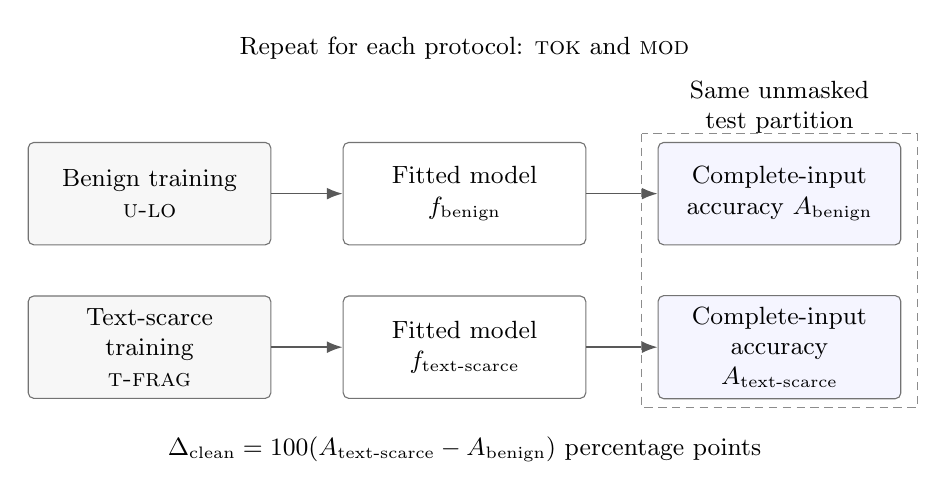
\begin{tikzpicture}[
  font=\small,
  box/.style={draw=black!55, rounded corners=2pt, align=center,
              minimum height=1.3cm, text width=2.8cm, inner sep=4pt},
  flow/.style={-{Latex[length=2mm]}, line width=0.6pt, draw=black!65}]
  \node[box, fill=black!3] (benign) at (0,0)
    {Benign training\\\textsc{u-lo}};
  \node[box, fill=black!3] (scarce) at (0,-1.95)
    {Text-scarce training\\\textsc{t-frag}};
  \node[box] (modelb) at (4,0) {Fitted model\\$f_{\rm benign}$};
  \node[box] (modelt) at (4,-1.95) {Fitted model\\$f_{\rm text\text{-}scarce}$};
  \node[box, fill=blue!4] (scoreb) at (8,0)
    {Complete-input\\accuracy $A_{\rm benign}$};
  \node[box, fill=blue!4] (scoret) at (8,-1.95)
    {Complete-input\\accuracy $A_{\rm text\text{-}scarce}$};
  \draw[flow] (benign) -- (modelb);
  \draw[flow] (scarce) -- (modelt);
  \draw[flow] (modelb) -- (scoreb);
  \draw[flow] (modelt) -- (scoret);
  \node[align=center] at (4,1.85)
    {Repeat for each protocol: \IMM{} and \FMM{}};
  \node[align=center, text width=3.2cm] at (8,1.1)
    {Same unmasked\\test partition};
  \draw[black!45, densely dashed] (6.25,0.76) rectangle (9.75,-2.72);
  \node[align=center] at (4,-3.25)
    {$\Delta_{\rm clean}=100(A_{\rm text\text{-}scarce}-A_{\rm benign})$
     percentage points};
\end{tikzpicture}

  \caption{\textbf{Clean-input change compares training histories on the same
  complete test inputs.} The design is repeated separately for token-level
  erasure (\IMM{}) and modality-level dropout (\FMM{}). Each protocol has
  its own benign-trained reference; architecture and optimization settings are
  shared, while model weights are fitted separately. Changes are paired by
  training-seed identifier before aggregation.}
  \label{fig:study_design}
\end{figure}

%======================================================================
\section{Experimental setup}\label{sec:setup}
%======================================================================

\subsection{Datasets and shared architecture}

% [data] provenance, verified
We evaluate on the three standard benchmarks for this task and verify the
provenance of every feature file. CMU-MOSI provides $1{,}284$ training,
$229$ validation and $686$ test utterances; CMU-MOSEI provides $16{,}326$,
$1{,}871$ and $4{,}659$; and CH-SIMS provides $1{,}368$, $456$ and $457$. All
three are used with the pre-extracted unaligned features distributed by the
MMSA toolkit, and each file's SHA-256 digest is checked against the value
published by that project before use. CMU-MOSI and CMU-MOSEI
carry sentiment labels in $[-3,3]$; CH-SIMS uses $[-1,1]$ and is in Chinese,
which additionally lets us test whether our findings depend on the language of
the text stream.

% [model] deliberately conventional, so the finding is not architecture-specific
We use a shared reconstruction-based fusion architecture to compare the two
training protocols. Each modality is encoded by a
two-layer transformer with learned positional embeddings and masked mean
pooling; per-modality reconstruction heads predict the pooled representation
of an absent modality from the surviving ones, supervised by the pooled
representations the same encoders produce on complete input; and a fusion
multilayer perceptron consumes the three pooled vectors together with explicit
availability flags. The text pathway is the one component we vary: instead of
consuming the stored features, a pretrained encoder (\texttt{bert-base} for
CMU-MOSI and CMU-MOSEI, \texttt{bert-base-chinese} for CH-SIMS,
\texttt{roberta-base} in Section~\ref{sec:modulators}) produces per-token
representations that enter the \emph{same} modality encoder the stored
features would have. Fine-tuning therefore changes how those $768$-dimensional
vectors are produced within the shared downstream architecture.

All modality encoders project their inputs to dimension $d=64$ and use
four attention heads with feed-forward width $4d$. Masked mean pooling is
followed by layer normalization. Residual and feed-forward dropout are $0.1$;
self-attention dropout in these modality encoders is zero. The pretrained
text model retains its own dropout configuration. Each reconstruction head
has two hidden layers of width $128$, GELU activations and dropout $0.1$.
The fusion network maps its $195$ inputs through widths $128$ and $64$ to a
scalar sentiment prediction. Holding this stack fixed makes the encoder and
missingness comparisons interpretable within one shared model family.

\subsection{Availability-gated reconstruction objective}

Let $\widetilde{x}_{ik}$ denote the corrupted stream for example $i$,
$a_{ik}$ indicate whether any valid position survives, and
$z_{ik}=E_k(\widetilde{x}_{ik})\in\mathbb{R}^{d}$ be its pooled encoding.
The reconstruction head $R_k$ receives the other streams' availability-gated
encodings and their flags:
\begin{align}
\widehat z_{ik} &= R_k\!\left([(a_{ij}z_{ij})_{j\ne k},(a_{ij})_{j\ne k}]\right),
\label{eq:reconstruction}\\
u_{ik} &= a_{ik}z_{ik}+(1-a_{ik})\widehat z_{ik},
\label{eq:availability_gate}\\
\widehat y_i &= F\!\left([u_{it},u_{ia},u_{iv},a_{it},a_{ia},a_{iv}]\right).
\label{eq:prediction}
\end{align}
In Equation~\eqref{eq:reconstruction}, brackets denote concatenation.
The gate in Equation~\eqref{eq:availability_gate} selects the representation
used by the fusion network and scalar head $F$ in Equation~\eqref{eq:prediction}.
A partially observed stream contributes its observed
encoding; a fully absent stream contributes its reconstruction. At clean
test time all availability flags equal one, so prediction uses the observed
encodings directly.

For a batch of $B$ examples, define $m_{ik}=1-a_{ik}$ and the detached
complete-input target $z^{\star}_{ik}=\operatorname{sg}(E_k(x_{ik}))$.
The training objective is
\begin{align}
\mathcal{L}_{\rm task} &= \frac{1}{B}\sum_{i=1}^{B}|\widehat y_i-y_i|,
\label{eq:task_loss}\\
\mathcal{L}_{\rm rec} &=
\frac{\displaystyle\sum_{i,k}m_{ik}\,
      \|\widehat z_{ik}-z^{\star}_{ik}\|_2^2/d}
     {\displaystyle\max(1,\sum_{i,k}m_{ik})},
\label{eq:reconstruction_loss}\\
\mathcal{L} &= \mathcal{L}_{\rm task}+0.5\mathcal{L}_{\rm rec}.
\label{eq:objective}
\end{align}
Equation~\eqref{eq:objective} combines sentiment regression
(Equation~\eqref{eq:task_loss}) with representation reconstruction
(Equation~\eqref{eq:reconstruction_loss}). The reconstruction term is zero
when the batch contains no fully absent
streams. Targets are recomputed with the current encoder parameters on the
complete training observations, without back-propagation through the target
branch. This branch remains in training mode, including dropout; it is not a
separate frozen teacher. Complete observations provide training supervision,
while inference uses only the supplied inputs and availability masks.

The comparison is between complete training protocols rather than isolated
gradient paths. The reconstruction loss is availability-gated: whole-modality
absence activates it whenever a stream is dropped, whereas partial temporal
erasure activates it only if no valid position survives. This fixed behaviour
is part of the operational difference induced by the two protocols.
Before restoration, a stream of length $L_k$ is fully absent with probability
$r_k^{L_k}$ under token-level erasure and $r_k$ under modality-level dropout.
For longer streams, these probabilities can differ substantially. The
reconstruction objective therefore receives different supervision frequencies
even though its coefficient and implementation remain fixed.

\subsection{Optimization, checkpoint selection and evaluation}

% [training] the leakage-avoiding detail that matters most
Optimisation uses AdamW with two parameter groups. The pretrained encoder is trained at
$2\times10^{-5}$ while the randomly initialised fusion stack uses
$10^{-3}$.
Training runs for at most $40$ epochs with early stopping on validation mean
absolute error, and validation is always performed under the \emph{training}
regime. Checkpoints are selected using validation MAE under that regime;
test scores are not used for selection. Each selected checkpoint is evaluated
on the test conditions described below. Batch size is $32$, weight decay is $10^{-4}$, and
gradients are clipped to norm $1$. Early stopping allows eight epochs without
an improvement of more than $10^{-5}$ in validation MAE. Validation averages
two corruption draws for each checkpoint evaluation.

% [protocol hygiene] the discipline that makes cross-method comparison valid
Both protocols use a shared masking implementation with random draws on CPU.
The reported results evaluate each trained model once on complete test inputs;
this evaluation applies no corruption. Archived incomplete-input evaluations
average five mask draws. Their hash seeds depended on the Python process, so
identical corrupted inputs across separate runs are not guaranteed. The
released driver uses stable digest seeds for future runs. Validation also
uses missingness, making its sampled masks part of the original checkpoint
selection procedure.

% [statistics and competitiveness]
Acc-2 is the fraction of correct positive-versus-negative predictions after
excluding test examples whose ground-truth sentiment equals zero; predictions
above zero are positive. MAE uses all test examples and clips predictions to
the dataset's label range. We report mean $\pm$ standard deviation over three
to five training seeds, using population standard deviations to describe the
observed runs. Changes are calculated within matched seed identifiers before
aggregation. These intervals describe variation across runs, rather than
confidence intervals or hypothesis tests.
Specifically, for matched seeds $s=1,\ldots,S$, we calculate
$\delta_s=100(A_{s,\mathrm{t\text{-}frag}}-A_{s,\mathrm{u\text{-}lo}})$,
then report $\bar\delta=S^{-1}\sum_s\delta_s$ and
$\sigma_\delta=[S^{-1}\sum_s(\delta_s-\bar\delta)^2]^{1/2}$.
Pairing preserves the correspondence between run identifiers; it does not
imply that independently executed runs used identical validation masks.
The sample-size study additionally holds each selected subset fixed across
training seeds, so its error bars describe training variation conditional on
that subset.

Table~\ref{tab:backbone} reports the benign-regime reference separately for
each protocol. This supplies the absolute accuracy and regression error from
which the text-scarce comparisons are calculated.

\begin{table}[t]
\centering
\caption{Clean-input performance under benign missingness training with BERT.
Acc-2 excludes neutral labels; MAE uses all examples. Values are mean $\pm$
standard deviation across five seeds for each dataset and protocol.}
\label{tab:backbone}
\small

\begin{tabular}{llcc}
\toprule
Dataset & Training protocol & Acc-2 $\uparrow$ & MAE $\downarrow$ \\
\midrule
CMU-MOSI & \tokenlevel{} & 0.835 $\pm$ 0.007 & 0.813 $\pm$ 0.024 \\
CMU-MOSI & \modlevel{} & 0.845 $\pm$ 0.007 & 0.728 $\pm$ 0.019 \\
CMU-MOSEI & \tokenlevel{} & 0.842 $\pm$ 0.012 & 0.531 $\pm$ 0.004 \\
CMU-MOSEI & \modlevel{} & 0.844 $\pm$ 0.006 & 0.525 $\pm$ 0.005 \\
CH-SIMS & \tokenlevel{} & 0.810 $\pm$ 0.011 & 0.403 $\pm$ 0.010 \\
CH-SIMS & \modlevel{} & 0.806 $\pm$ 0.018 & 0.411 $\pm$ 0.021 \\
\bottomrule
\end{tabular}

\end{table}

%======================================================================
\section{Token-level training erodes clean-input performance}\label{sec:granularity}
%======================================================================

\subsection{Clean-input classification and regression}

% [core claim] the two protocols are not interchangeable
The two protocols produce markedly different clean-input outcomes.
Table~\ref{tab:degradation} reports $\degr$, the difference in clean-input
accuracy between text-scarce and benign training. The nominal rate schedules
are matched across protocols. Under \tokenlevel{} erasure the loss reaches
$20.8$ points on CMU-MOSI with BERT and $27.7$ with RoBERTa. Under \modlevel{}
absence the same comparison costs $0.8$ and $2.0$ points respectively. The
direction is consistent across every dataset and both text encoders:
\tokenlevel{} erasure changes clean-input accuracy substantially more than
\modlevel{} absence.

% [what the measurement means] and why it is not a robustness result
Because $\degr$ is measured on complete input, it is distinct from robustness
under a particular test-time mask. A system with $\degr=-20.8$ has lost
complete-input task accuracy after missingness training. Standard evaluations
that test a missingness-trained model only on corrupted inputs do not expose
this quantity.

Regression error corroborates the classification result in the full-data BERT
experiments (Table~\ref{tab:mae_change}). Text-scarce token-level training
increases MAE by $0.510$ on CMU-MOSI, $0.078$ on CMU-MOSEI and $0.039$ on
CH-SIMS. With modality-level training, the respective changes are $0.063$,
$0.016$ and $-0.021$. Thus the token-level result also appears in distance from the
annotated sentiment score, beyond whether a prediction crosses the polarity
boundary. On CH-SIMS, modality-level MAE improves even though the accuracy
change is small, illustrating that polarity and sentiment magnitude capture
different aspects of the output. MAE magnitudes should be compared within a
dataset because the label ranges differ.

\begin{table}[t]
\centering
\caption{Clean-input MAE under benign and text-scarce training with BERT on
the full datasets. A positive change indicates higher error. Changes are
mean $\pm$ population standard deviation across five matched seeds; the two
regime columns show mean MAE. All values use the original sentiment scale.}
\label{tab:mae_change}
\small

\begin{tabular}{llccc}
\toprule
Dataset & Protocol & Benign & Text-scarce & MAE change $\downarrow$ \\
\midrule
CMU-MOSI & \tokenlevel{} & 0.813 & 1.323 & +0.510 $\pm$ 0.108 \\
CMU-MOSI & \modlevel{} & 0.728 & 0.791 & +0.063 $\pm$ 0.040 \\
CMU-MOSEI & \tokenlevel{} & 0.531 & 0.609 & +0.078 $\pm$ 0.008 \\
CMU-MOSEI & \modlevel{} & 0.525 & 0.541 & +0.016 $\pm$ 0.011 \\
CH-SIMS & \tokenlevel{} & 0.403 & 0.443 & +0.039 $\pm$ 0.020 \\
CH-SIMS & \modlevel{} & 0.411 & 0.391 & -0.021 $\pm$ 0.026 \\
\bottomrule
\end{tabular}

\end{table}

\subsection{Dependence on the nominal text-erasure rate}

% [dose-response] the shape of the effect, and the threshold
The rate sweep locates the range where clean-input performance changes.
Figure~\ref{fig:dose} varies the
training text-erasure rate from $0$ to $0.9$ on CMU-MOSI and CH-SIMS. Below
approximately $0.5$, the two curves are close. At higher rates they separate
sharply: \tokenlevel{} erasure
reaches $0.575$ accuracy on CMU-MOSI, a drop of $26.3$ points
from the zero-erasure baseline, while \modlevel{} absence loses $7.8$. CH-SIMS
has its largest token-level decrease at rate $0.8$ ($12.3$ points), compared
with a largest modality-level decrease of $6.5$ points at rate $0.9$.
For descriptive comparison, we define onset as the first tested rate whose
mean accuracy is more than two percentage points below that protocol's
rate-zero reference. This occurs at $0.5$ on CMU-MOSI and $0.6$ on CH-SIMS
under token-level training. The criterion identifies points on the tested
grid, rather than a fitted change point. Audio and video rates remain $0.1$
throughout, including at the text-rate-zero reference.

\begin{figure}[t]
  \centering
  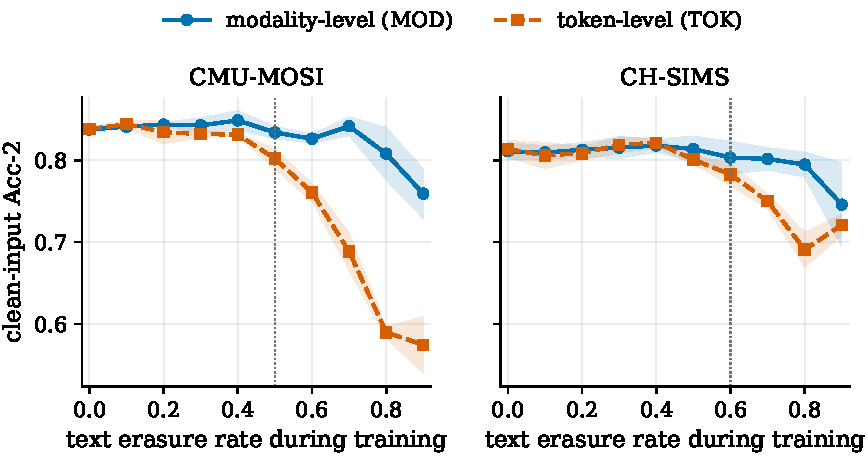
\includegraphics[width=\linewidth]{figs/dose_response.pdf}
  \caption{\textbf{Training protocols separate as nominal text erasure increases.}
  Clean-input accuracy after training under \tokenlevel{} erasure (\IMM{},
  orange) or \modlevel{} absence (\FMM{}, blue) at a given text erasure rate.
  Dotted lines mark the first tested token-level rate with more than a two-point
  decrease from the text-rate-zero reference: $0.5$ and $0.6$, respectively.
  Shaded bands show $\pm 1$ standard deviation over three seeds.}
  \label{fig:dose}
\end{figure}

% [context] comparison with missing rates used in prior evaluations
The onset lies within rates used in prior evaluations. EMT-DLFR evaluates
rates from $0.1$ to $1.0$ on CMU-MOSI and CMU-MOSEI, and up to $0.5$ on
CH-SIMS~\cite{emtdlfr}; MRCF evaluates intra-modal missingness from $0.0$ to
$0.9$~\cite{mrcf}. The observed onset rates therefore fall within
evaluation ranges used in prior studies.

\subsection{Unknown-token substitution control}

% [operator check] replicate with the operation used in prior work
The operator check repeats the comparison with the text substitution used in
prior work. Our
\tokenlevel{} operator removes a masked position from the attention mask, so
the token becomes invisible. EMT-DLFR instead ``replaces the original token
with the [UNK] token in BERT vocabulary''~\cite{emtdlfr}, leaving the position
visible but uninformative. Repeating the CMU-MOSI experiment with that
substitution in place of removal gives a clean-input change of $-29.6$ points
($0.828 \rightarrow 0.532$ \cleanacc{}, three seeds) against $-20.8$ for
removal. Substituting an unknown-token embedding at most positions produces a
larger clean-input change than making those positions invisible. The
observation is therefore not specific to removal from the attention mask.

\begin{table}[t]
\centering
\caption{Clean-input change $\degr$ after text-scarce rather than benign
missingness training. The benign Acc-2 column is the token-level reference;
modality-level changes use their own benign reference. Values are mean $\pm$
standard deviation of paired-seed changes, with five seeds for full-data BERT
and three for subsampled BERT and RoBERTa.}
\label{tab:degradation}
\small
\resizebox{\linewidth}{!}{
\begin{tabular}{llccc}
\toprule
 & & benign & \multicolumn{2}{c}{clean-input Acc-2 change (pts)} \\
\cmidrule(lr){4-5}
Text encoder & Dataset & Acc-2 & \tokenlevel{} & \modlevel{} \\
\midrule
BERT & CMU-MOSI & 0.835 $\pm$ 0.007 & -20.8 $\pm$ 7.9 & -0.8 $\pm$ 1.6 \\
 & CMU-MOSEI ($n{=}1284$) & 0.839 $\pm$ 0.005 & -12.7 $\pm$ 4.2 & -1.7 $\pm$ 0.4 \\
 & CH-SIMS & 0.810 $\pm$ 0.011 & -4.6 $\pm$ 2.3 & +0.1 $\pm$ 2.0 \\
 & CMU-MOSEI & 0.842 $\pm$ 0.012 & -3.2 $\pm$ 1.1 & -0.7 $\pm$ 0.8 \\
\addlinespace
RoBERTa & CMU-MOSI & 0.853 $\pm$ 0.011 & -27.7 $\pm$ 3.7 & -2.0 $\pm$ 2.4 \\
 & CMU-MOSEI ($n{=}1284$) & 0.838 $\pm$ 0.002 & -18.1 $\pm$ 0.7 & -2.2 $\pm$ 2.2 \\
\bottomrule
\end{tabular}
}
\end{table}

%======================================================================
\section{What modulates the clean-input change}\label{sec:modulators}
%======================================================================

\subsection{Training-set size}

% [size] the factor that dominates, isolated by subsampling
Training-set size strongly modulates the magnitude of the clean-input change.
The effect is
much larger on CMU-MOSI ($20.8$ points) than on full CMU-MOSEI ($3.2$), and
those datasets differ in many ways. We therefore examined training-set size
through nested CMU-MOSEI subsets while holding features, architecture, protocol and
full-training-set normalization statistics fixed. The subsets are nested
prefixes of one seeded permutation, shared across training seeds.
Figure~\ref{fig:size} shows the result: the overall change grows as data
shrink, from $3.2$ points at
$16{,}326$ training examples to $12.7$ at $1{,}284$, a fourfold increase
over a $12.7\times$ reduction in data. Two features of that curve matter. The
benign-regime line is flat across the whole range ($0.839$ to $0.844$), so
the observed size sensitivity is concentrated in the text-scarce regime.
The intermediate values are not strictly monotonic. At CMU-MOSI's exact
training-set size, CMU-MOSEI reaches $12.7$ points against CMU-MOSI's $20.8$
points. The within-CMU-MOSEI comparison supports a sample-size association,
while the remaining cross-dataset difference also reflects corpus variation.

\subsection{Text encoder and corpus variation}

% [encoder] generality, and the counter-intuitive direction
The encoder comparison uses model-specific tokenisation with consistent
input casing. The benchmarks store BERT WordPiece indices, so we regenerate
RoBERTa identifiers from the raw transcripts. Every CMU-MOSI transcript is
upper-cased; we lowercase these inputs before applying RoBERTa's
case-sensitive tokenizer. Table~\ref{tab:tokenization_audit} quantifies the
result at the shared 50-token limit. On the training partition, lowercasing
reduces mean retained RoBERTa length from $20.49$ to $14.81$ tokens; BERT
averages $14.78$. True truncation falls from $3.58\%$ to $0.62\%$, compared with
$0.55\%$ for BERT. Here truncation means that the sequence exceeds the limit
before clipping; sequences exactly at the limit are counted separately in
the released audit. Lowercasing aligns length exposure more closely while
retaining each encoder's own tokenizer.

The clean-input protocol contrast persists with RoBERTa
(Figure~\ref{fig:encoders}).
\tokenlevel{} erasure changes RoBERTa accuracy by $-27.7$ points on CMU-MOSI and $-18.1$
on size-matched CMU-MOSEI, while \modlevel{} absence costs $2.0$ and $2.2$.
RoBERTa begins from a higher clean baseline than BERT in this setting ($0.853$
against $0.835$) and shows the larger clean-input change.

\begin{table}[t]
\centering
\caption{CMU-MOSI tokenisation audit at a 50-token limit, including special
tokens. Length is the mean retained token count; truncated is the percentage
whose untruncated length exceeds 50. Lowercased RoBERTa identifiers and masks
match the experiment cache on all three partitions.}
\label{tab:tokenization_audit}
\small
\begin{tabular}{lrrrr}
\toprule
 & \multicolumn{2}{c}{Training} & \multicolumn{2}{c}{Test} \\
\cmidrule(lr){2-3}\cmidrule(lr){4-5}
Tokenizer / input & Length & Trunc. (\%) & Length & Trunc. (\%) \\
\midrule
BERT-uncased & 14.78 & 0.55 & 16.50 & 2.04 \\
RoBERTa / original & 20.49 & 3.58 & 22.50 & 5.54 \\
RoBERTa / lowercase & 14.81 & 0.62 & 16.54 & 1.90 \\
\bottomrule
\end{tabular}

\end{table}

% [negative result] the hypothesis we had and discarded
The size-matched results also retain a corpus difference: the change is
$12.7$ points on CMU-MOSEI and $20.8$ on CMU-MOSI. Subsampling therefore
accounts for part of the contrast between the full datasets while preserving
variation associated with their content and feature distributions.

\begin{figure}[!htbp]
  \centering
  \begin{subfigure}{0.85\linewidth}
    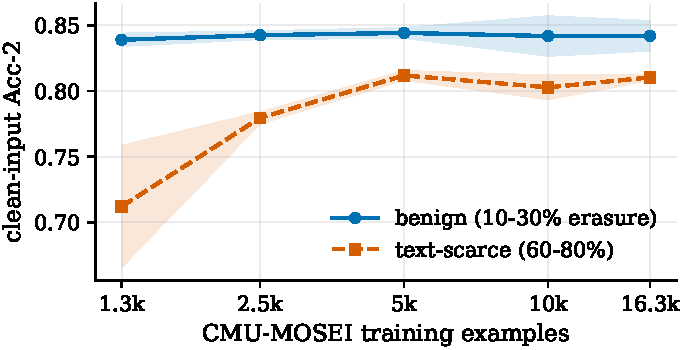
\includegraphics[width=\linewidth]{figs/size_response.pdf}
    \caption{Training-set size}\label{fig:size}
  \end{subfigure}\par\medskip
  \begin{subfigure}{0.85\linewidth}
    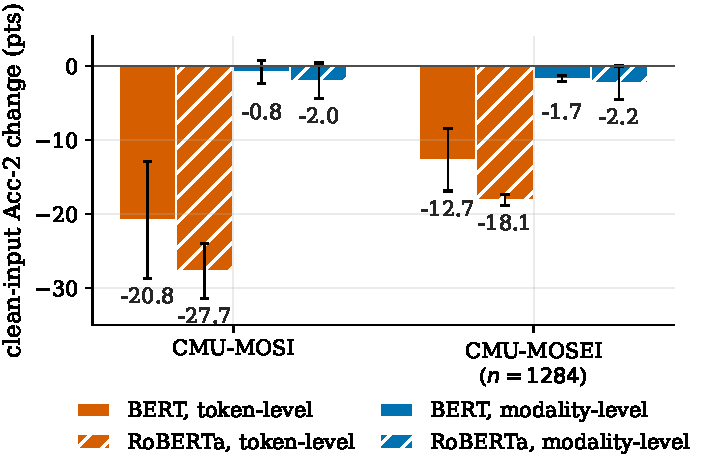
\includegraphics[width=\linewidth]{figs/encoders.pdf}
    \caption{Text encoder and training protocol}\label{fig:encoders}
  \end{subfigure}
  \caption{\textbf{Data scale and text encoder modulate clean-input change.}
  (\subref{fig:size}) CMU-MOSEI subsampling; shading shows $\pm 1$ standard
  deviation over three seeds at each subsample size and five at full size.
  Normalization uses the full training partition.
  (\subref{fig:encoders}) Mean paired-seed clean-input changes with $\pm 1$
  standard deviation: five seeds for BERT on CMU-MOSI, three otherwise.
  Both text encoders retain substantially more complete-input accuracy under
  \modlevel{} absence.}
  \label{fig:modulators}
\end{figure}

%======================================================================
\section{Mitigation}\label{sec:mitigation}
%======================================================================

% [result] one intervention works, and it is the granularity change
The modality-level training protocol keeps clean-input accuracy close to its
benign-regime reference. Table~\ref{tab:mitigations}
compares three interventions against the \tokenlevel{} baseline. Training with
\modlevel{} dropout (M1) moves the clean-input change from
$-20.8$ points to $-0.2$ on CMU-MOSI and from $-4.6$ to $+0.9$ on CH-SIMS, while
maintaining benign-regime accuracy. Freezing the
embedding layer and the lower six transformer blocks (M2) and cutting the
encoder learning rate fourfold (M3) do not provide the same recovery.

% [interpretation] the intervention outcome and its evaluation use
M1 changes the observation distribution and its associated reconstruction
exposure. In this architecture, that complete training protocol retains
clean-input accuracy more consistently than the two tested changes to encoder
adaptation. Its clean-input result makes it a useful comparator when selecting
a training protocol. Selection for deployment should additionally compare
the candidates on a common suite of expected missing-input conditions.

\begin{table}[t]
\centering
\caption{Clean-input performance under three interventions. Changing the
training protocol to \modlevel{} dropout (M1) preserves accuracy; freezing
lower layers (M2) and reducing the encoder learning rate (M3) do not.
Values are mean $\pm$ standard deviation over five baseline seeds and three
intervention seeds; changes are paired by seed.}
\label{tab:mitigations}
\small
\resizebox{\linewidth}{!}{
\begin{tabular}{llccc}
\toprule
 & & \multicolumn{2}{c}{clean-input Acc-2 $\uparrow$} & \\
\cmidrule(lr){3-4}
Dataset & Training scheme & benign & text-scarce & change (pts) \\
\midrule
CMU-MOSI & \tokenlevel{} baseline & 0.835 $\pm$ 0.007 & 0.627 $\pm$ 0.076 & -20.8 $\pm$ 7.9 \\
 & M1: \modlevel{} training & 0.839 $\pm$ 0.006 & 0.837 $\pm$ 0.004 & -0.2 $\pm$ 0.3 \\
 & M2: freeze embed.\ $+$ 6 blk. & 0.823 $\pm$ 0.007 & 0.586 $\pm$ 0.028 & -23.7 $\pm$ 2.2 \\
 & M3: encoder LR $5\times10^{-6}$ & 0.833 $\pm$ 0.011 & 0.595 $\pm$ 0.026 & -23.9 $\pm$ 3.7 \\
\addlinespace
CH-SIMS & \tokenlevel{} baseline & 0.810 $\pm$ 0.011 & 0.764 $\pm$ 0.022 & -4.6 $\pm$ 2.3 \\
 & M1: \modlevel{} training & 0.805 $\pm$ 0.009 & 0.814 $\pm$ 0.013 & +0.9 $\pm$ 0.7 \\
 & M2: freeze embed.\ $+$ 6 blk. & 0.828 $\pm$ 0.006 & 0.759 $\pm$ 0.029 & -6.9 $\pm$ 2.4 \\
 & M3: encoder LR $5\times10^{-6}$ & 0.822 $\pm$ 0.002 & 0.770 $\pm$ 0.018 & -5.2 $\pm$ 1.6 \\
\bottomrule
\end{tabular}
}
\end{table}

%======================================================================
\FloatBarrier
\section{Discussion and limitations}\label{sec:limitations}
%======================================================================

\subsection{Implications for evaluation and training}

The exposure measurement identifies two operational differences behind a
shared nominal missing-rate schedule. Under text-scarce training on CMU-MOSI,
modality-level dropout provides intact text in $30.33\%$ of draws, compared
with $0.04\%$ for token-level erasure. It also supplies $1.070$ rather than
$0.033$ reconstruction-eligible pairs per utterance
(Table~\ref{tab:masking_exposure}). Intact-input exposure and reconstruction
exposure therefore vary together in the implemented comparison. These
measurements explain what changes between protocols; the accuracy experiments
measure the resulting system-level outcome. Identifying each exposure's
individual contribution requires independently controlling the reconstruction
objective and the observation distribution.

The factorial control in Section~\ref{sec:control_cuda} removes auxiliary
reconstruction supervision while retaining the prediction architecture.
At zero reconstruction weight, clean-input accuracy changes by
$-22.96\pm8.56$ points under token-level training and $-1.10\pm2.61$ under
modality-level training. Thus the observed protocol contrast also occurs
without that auxiliary objective. Reconstruction-based imputation and the
observation distributions still differ across protocols, so the control
isolates loss-weight sensitivity rather than every consequence of missingness.

A practical evaluation should retain the clean test condition for every
missingness-trained checkpoint. Reporting its absolute score, change from a
specified training reference, and missing-input scores gives distinct views
of retained capability and tolerance to unavailable inputs. This is especially
useful when tuning corruption rates: a setting selected solely for performance
on corrupted observations may give a different trade-off from one selected
for a deployment mixture that includes complete inputs. The present results
characterize the clean-input side of that trade-off; choosing a deployment
policy also requires the expected test-time observation patterns.

The intervention results guide which training choices deserve direct testing.
Reducing encoder plasticity through the two tested settings does not recover
the token-level baseline, whereas changing the observation protocol does.
This favors evaluating protocol choice early in model development. It also
motivates a more targeted mechanistic experiment: vary corruption granularity
while independently controlling intact-text exposure and imputation, then compare both
complete-input outcomes and the representations along the text and fusion
paths. Such a design would distinguish which components of the current
operational difference contribute most to the measured change.

\subsection{Scope of the evidence}

The evidence is bounded to masked-language-model text pathways and one fusion
architecture. The comparison evaluates complete training protocols, including
their availability-gated reconstruction behaviour, rather than attributing the
effect to a single layer or gradient path. Extending clean-input performance to
decoder-only text towers and published missing-modality architectures is the
next step toward a broader protocol benchmark. The three-to-five-seed design
supports descriptive comparisons; the rate-grid onset criterion and the
single fixed subset at each sample size do not establish population-level
thresholds or uncertainty over training-set selection.

%======================================================================
\section{Conclusion}\label{sec:conclusion}
%======================================================================

We have compared missingness-training protocols through their clean-input
changes relative to benign training. Across three sentiment benchmarks,
high-rate \tokenlevel{} erasure changed complete-input accuracy by up to
$-27.7$ points, while \modlevel{} absence preserved substantially more of that
capability in the shared reconstruction-based architecture. On the tested rate
grids, token-level declines first pass two percentage points at $50$--$60\%$
text erasure. Smaller training subsets generally show larger changes, and the
effect appears with BERT, RoBERTa and \texttt{[UNK]} substitution. A separate
five-seed control reproduces the protocol contrast at both tested
reconstruction-loss weights, including zero. Together,
these results establish clean-input performance as a consequential outcome of
missingness-training protocol choice. Reporting the protocol alongside the
nominal rate, and evaluating complete inputs alongside corrupted inputs,
makes this distinction visible in multimodal evaluation.

\clearpage
\appendix
\setcounter{table}{0}
\section{Five-seed auxiliary-loss control}\label{sec:control_cuda}

% [design] fixed factorial intervention and selection rule
We test whether auxiliary reconstruction supervision is required for the
clean-input protocol contrast. The study crosses two training protocols,
two regimes (benign and text-scarce), two reconstruction-loss weights
($\lambda_{\rm rec}=0$ and $0.5$), and five matched seeds, giving 40 runs on
the full CMU-MOSI training partition. The architecture, batch size, learning
rates, 40-epoch maximum and eight-epoch patience remain fixed. Checkpoint
selection uses validation MAE under the training regime, averaged over two
fixed mask draws. All five seeds enter every comparison. Reconstruction heads and the
detached complete-input target forward pass remain active at both weights;
the intervention removes the auxiliary objective, not imputation from the
prediction pathway.

% [provenance] separate execution environment and replicated inputs
These runs use an RTX PRO 6000 Blackwell GPU, PyTorch 2.8.0 with CUDA 12.8,
Transformers 4.57.6, BF16 autocast and scaled dot-product attention.
Dataset and initial BERT-weight hashes match the local control inputs.
The stable evaluation-seed implementation is shared across all 40 runs.
This study is analysed separately from the archived experiments and the
Metal pilot below; it does not isolate the effect of changing the historical
validation-mask seed implementation from other runtime differences.

% [evidence] within-protocol changes and variation
The clean-input contrast persists at both loss weights
(Table~\ref{tab:control_cuda}). At zero loss weight,
token-level training changes Acc-2 by $-22.96\pm8.56$ percentage points,
compared with $-1.10\pm2.61$ for modality-level training. At weight $0.5$,
the corresponding changes are $-16.52\pm5.09$ and $-0.61\pm3.10$ points.
Token-level accuracy decreases in all five seeds at each weight. MAE gives
the same ordering: increases of $0.553$ versus $0.087$ at weight zero and
$0.458$ versus $0.130$ at weight $0.5$
(Table~\ref{tab:control_cuda_mae}).

\begin{table}[!htbp]
\centering
\caption{Complete-input Acc-2 in the separate CUDA factorial study. Values
are mean $\pm$ population standard deviation over five seeds per condition.
The last column uses within-seed text-scarce-minus-benign differences.}
\label{tab:control_cuda}
\small
\resizebox{\linewidth}{!}{\begin{tabular}{lrccc}
\toprule
Training & $\lambda_{\rm rec}$ & Benign Acc-2 $\uparrow$ & Text-scarce Acc-2 $\uparrow$ & $\Delta_{\rm clean}$ (pp) \\
\midrule
\tokenlevel{} & 0.0 & 0.833 $\pm$ 0.007 & 0.604 $\pm$ 0.080 & -22.96 $\pm$ 8.56 \\
\tokenlevel{} & 0.5 & 0.829 $\pm$ 0.006 & 0.664 $\pm$ 0.051 & -16.52 $\pm$ 5.09 \\
\modlevel{} & 0.0 & 0.835 $\pm$ 0.005 & 0.824 $\pm$ 0.026 & -1.10 $\pm$ 2.61 \\
\modlevel{} & 0.5 & 0.836 $\pm$ 0.007 & 0.830 $\pm$ 0.026 & -0.61 $\pm$ 3.10 \\
\bottomrule
\end{tabular}
}
\end{table}

\begin{table}[!htbp]
\centering
\caption{Complete-input MAE for the same 40 CUDA runs, reported as mean
$\pm$ population standard deviation over five seeds per condition. Changes
are computed within seed; positive changes indicate greater prediction error.}
\label{tab:control_cuda_mae}
\small
\resizebox{\linewidth}{!}{\begin{tabular}{lrccc}
\toprule
Training & $\lambda_{\rm rec}$ & Benign MAE $\downarrow$ & Text-scarce MAE $\downarrow$ & MAE change $\downarrow$ \\
\midrule
\tokenlevel{} & 0.0 & 0.793 $\pm$ 0.036 & 1.346 $\pm$ 0.105 & +0.553 $\pm$ 0.117 \\
\tokenlevel{} & 0.5 & 0.810 $\pm$ 0.012 & 1.268 $\pm$ 0.071 & +0.458 $\pm$ 0.068 \\
\modlevel{} & 0.0 & 0.752 $\pm$ 0.011 & 0.840 $\pm$ 0.054 & +0.087 $\pm$ 0.053 \\
\modlevel{} & 0.5 & 0.736 $\pm$ 0.008 & 0.866 $\pm$ 0.087 & +0.130 $\pm$ 0.094 \\
\bottomrule
\end{tabular}
}
\end{table}

% [interpretation] paired protocol contrast and coefficient interaction
For each seed, we subtract the modality-level clean-input change from the
token-level change. This protocol contrast is $-21.86\pm11.16$ points at
weight zero and $-15.91\pm6.25$ at weight $0.5$; it is negative in every
seed at both weights. The coefficient interaction, defined as the latter
contrast minus the former, is $+5.95\pm14.65$ points. Its seed-level values
range from $-19.36$ to $+22.41$ points, so the mean attenuation does not imply
a consistent benefit from the auxiliary objective. The MAE contrast is
$0.466\pm0.169$ at zero weight and $0.327\pm0.085$ at weight $0.5$,
with an interaction of $-0.138\pm0.215$.
The stable result is that the protocol contrast remains when auxiliary
reconstruction supervision is removed. The remaining protocol differences include the
observation distribution and availability-dependent prediction path within
this architecture.

\FloatBarrier
\setcounter{table}{0}
\section{Supplementary Metal pilot}\label{sec:control_pilot}

We examine auxiliary-loss sensitivity with a matched single-seed control on
the full CMU-MOSI training partition. Both runs use token-level text-scarce
training, seed zero and the same reconstruction architecture, with
$\lambda_{\rm rec}=0$ or $0.5$. The reconstruction heads remain in the
prediction path, and both runs retain the complete-input target forward pass.
The intervention changes the auxiliary loss coefficient while preserving
those computations. Validation uses deterministic masks under the training
regime, with the learning rates, batch size and stopping rule of
Section~\ref{sec:setup}.

The pilot uses PyTorch 2.14.0 and Transformers 4.57.6 on Apple Metal, with
full-precision computation and eager BERT attention to support attention
dropout. We report this local study separately from the archived CUDA results.
Both runs stop after 12 epochs and select the fourth epoch by validation MAE.
Table~\ref{tab:control_pilot} reports their complete-input outcomes. Removing
the auxiliary loss gives $54.42\%$ accuracy, compared with $57.32\%$ at weight
$0.5$; MAE is $1.415$ and $1.381$, respectively. Thus loss removal does not
improve clean-input performance for this seed and training condition.
This pilot measures auxiliary-loss sensitivity at a fixed text-scarce
regime. The complete five-seed, two-regime comparison is reported separately
in Section~\ref{sec:control_cuda} using a consistent CUDA runtime.

\begin{table}[!htbp]
\centering
\caption{Single-seed CMU-MOSI auxiliary-loss pilot under token-level text-scarce
training. Acc-2 and MAE use complete test inputs. Epoch indices are one-based.
Both conditions use the same local Metal runtime and reconstruction architecture.}
\label{tab:control_pilot}
\small
\begin{tabular}{rrrr}
\toprule
Rec. coefficient & Clean Acc-2 $\uparrow$ & Clean MAE $\downarrow$ & Selected epoch \\
\midrule
0.0 & 0.544 & 1.415 & 4 \\
0.5 & 0.573 & 1.381 & 4 \\
\bottomrule
\end{tabular}

\end{table}

We additionally evaluate both selected checkpoints on common missing-input
suites (Table~\ref{tab:control_common_eval}). Each suite uses the text-scarce
rate distribution, five deterministic mask repetitions and the same test
ordering and batch size for both checkpoints. Under token-erased test inputs,
mean accuracy is $55.21\%$ at weight zero and $58.26\%$ at weight $0.5$.
Under whole-modality dropout, both obtain $53.90\%$ accuracy, with MAE $1.435$
and $1.423$, respectively. The coefficient comparison therefore depends on
the evaluation condition. Both models in this pilot were trained with
token-level erasure; the suites compare auxiliary-loss settings under shared
test conditions rather than comparing the two training protocols.

\begin{table}[!htbp]
\centering
\caption{Common-suite evaluation of the two pilot checkpoints. Both models
were trained with token-level text-scarce missingness. Each test operator uses
the text-scarce nominal rate distribution; values are means over five mask
repetitions, not repeated training seeds.}
\label{tab:control_common_eval}
\small
\begin{tabular}{rlrr}
\toprule
Rec. coefficient & Test operator & Acc-2 $\uparrow$ & MAE $\downarrow$ \\
\midrule
0.0 & \tokenlevel{} & 0.552 & 1.412 \\
0.0 & \modlevel{} & 0.539 & 1.435 \\
0.5 & \tokenlevel{} & 0.583 & 1.371 \\
0.5 & \modlevel{} & 0.539 & 1.423 \\
\bottomrule
\end{tabular}

\end{table}

\FloatBarrier
\section*{CRediT authorship contribution statement}
\textbf{Zehao Li}: Methodology, Software, Formal analysis,
Writing -- original draft, Writing -- review \& editing.

\section*{Declaration of competing interest}
The author declares no known competing financial interests or personal
relationships that could have appeared to influence the work reported in this
paper.

\section*{Data availability}
All datasets used in this study are publicly available. CMU-MOSI~\cite{mosi},
CMU-MOSEI~\cite{mosei} and CH-SIMS~\cite{mmsa} were obtained
as the pre-extracted unaligned feature files distributed by the MMSA toolkit;
the SHA-256 digest of every file used is recorded in the released code and
checked before use. The manuscript source, experiment code, per-run results
and reproduction instructions are available in the
\href{https://github.com/Yed-13/Token-Level-Missingness-Training-Can-Erode-Clean-Input-Performance-in-Multimodal-Learnin}{public repository}.

\bibliographystyle{elsarticle-num}
\bibliography{refs}

\end{document}
